\begin{figure}[!ht]
    % \centering
    \subfloat[Intruder]{
        \label{Intruder}
        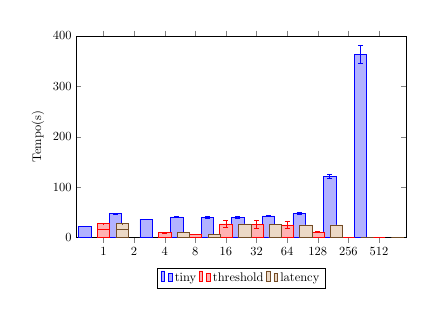
\begin{tikzpicture}[scale=0.45, baseline]
        \begin{axis}[
            width=0.9 \linewidth,
            height=0.6 \linewidth,
            %media de tempo intruder
            ybar=5pt,
            %enlargelimits=0.10,
            legend style={at={(0.5,-0.15)}, anchor=north, legend columns=-1},
            ylabel=Tempo(s),
            symbolic x coords={1, 2, 4, 8, 16, 32, 64, 128, 256, 512},
            xtick=data,
            ymin=0,
            ymax=400,
            bar width=10pt,
            % nodes near coords,
            nodes near coords align={vertical},
        ]
        \addplot+[error bars,y dir=both, y explicit] coordinates {
            (1,22.52)+-(1,0.13) (2,47.52)+-(2,1.02) (4,36.42)+-(4,0.57) (8,41.17)+-(8,1.22) (16,40.32)+-(16,1.21)
            (32,40.14)+-(32,2.42) (64,42.99)+-(64,1.48) (128,47.67)+-(128,2.37) (256,121.10)+-(256,4.24) (512,363.61)+-(512,17.08)}; %orininal
        \addplot+[error bars,y dir=both, y explicit] coordinates {
            (1,27.79)+-(1,0.15) (1,16.67)+-(2,0.18) (4,10.27)+-(4,0.86) (8,6.64)+-(8,0.34) (16,27.12)+-(16,7.19)
            (32,26.32)+-(32,7.19) (64,25.30)+-(64,7.72) (128,11.30)+-(128,0.42) (256,0.00)+-(256,0.0) (512,0.00)+-(512,0.0)}; %threshold
        \addplot+[error bars,y dir=both, y explicit] coordinates {
            (1,27.79)+-(1,0.13) (1,16.67)+-(2,0.13) (4,10.27)+-(4,0.13) (8,6.64)+-(8,0.13) (16,27.12)+-(16,0.13)
            (32,26.32)+-(32,0.13) (64,25.30)+-(64,0.13) (128,24.95)+-(128,0.13) (256,0.00)+-(256,0.13) (512,0.00)+-(512,0.13)}; %latency
        % \addplot coordinates {(1,405) (2,365) (4,338) (8,305) (16,263) (32,238) (64,225)}; %mainboard old
        \legend {tiny, threshold, latency}
        \end{axis}
        \end{tikzpicture}
    }
    \subfloat[Intruder]{
        \label{Intruder}
        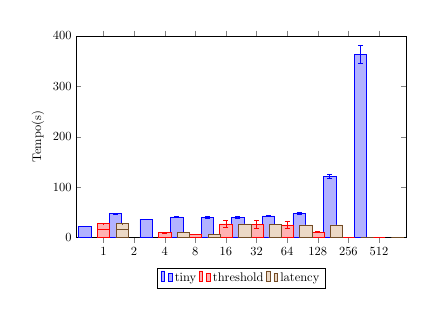
\begin{tikzpicture}[scale=0.45, baseline]
        \begin{axis}[
            width=0.9 \linewidth,
            height=0.6 \linewidth,
            %media de tempo intruder
            ybar=5pt,
            %enlargelimits=0.10,
            legend style={at={(0.5,-0.15)}, anchor=north, legend columns=-1},
            ylabel=Tempo(s),
            symbolic x coords={1, 2, 4, 8, 16, 32, 64, 128, 256, 512},
            xtick=data,
            ymin=0,
            ymax=400,
            bar width=10pt,
            % nodes near coords,
            nodes near coords align={vertical},
        ]
        \addplot+[error bars,y dir=both, y explicit] coordinates {
            (1,22.52)+-(1,0.13) (2,47.52)+-(2,1.02) (4,36.42)+-(4,0.57) (8,41.17)+-(8,1.22) (16,40.32)+-(16,1.21)
            (32,40.14)+-(32,2.42) (64,42.99)+-(64,1.48) (128,47.67)+-(128,2.37) (256,121.10)+-(256,4.24) (512,363.61)+-(512,17.08)}; %orininal
        \addplot+[error bars,y dir=both, y explicit] coordinates {
            (1,27.79)+-(1,0.15) (1,16.67)+-(2,0.18) (4,10.27)+-(4,0.86) (8,6.64)+-(8,0.34) (16,27.12)+-(16,7.19)
            (32,26.32)+-(32,7.19) (64,25.30)+-(64,7.72) (128,11.30)+-(128,0.42) (256,0.00)+-(256,0.0) (512,0.00)+-(512,0.0)}; %threshold
        \addplot+[error bars,y dir=both, y explicit] coordinates {
            (1,27.79)+-(1,0.13) (1,16.67)+-(2,0.13) (4,10.27)+-(4,0.13) (8,6.64)+-(8,0.13) (16,27.12)+-(16,0.13)
            (32,26.32)+-(32,0.13) (64,25.30)+-(64,0.13) (128,24.95)+-(128,0.13) (256,0.00)+-(256,0.13) (512,0.00)+-(512,0.13)}; %latency
        % \addplot coordinates {(1,405) (2,365) (4,338) (8,305) (16,263) (32,238) (64,225)}; %mainboard old
        \legend {tiny, threshold, latency}
        \end{axis}
        \end{tikzpicture}
    }
    
    \centering
    \subfloat[sparselong]{
    \label{tsparselong}
    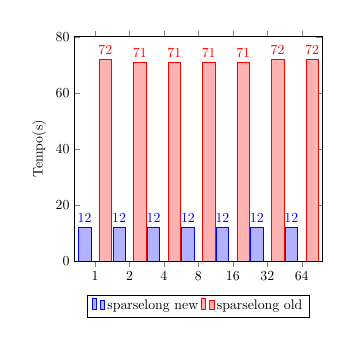
\begin{tikzpicture}[scale=0.5, baseline]
    \begin{axis}[
    width=0.65 \linewidth,
    height=0.6 \linewidth,
    ybar=6pt,
%    enlargelimits=0.12,
    legend style={at={(0.5,-0.15)}, anchor=north, legend columns=-1},
    ylabel=Tempo(s),
    symbolic x coords={1, 2, 4, 8, 16, 32, 64},
    xtick=data,
    ymin=0,
    ymax=80,
    bar width=9pt,
    nodes near coords,
    nodes near coords align={vertical},
    ]

    \addplot coordinates {(1,12) (2,12) (4,12) (8,12) (16,12) (32,12) (64,12)}; %sparselong new
    \addplot coordinates {(1,72) (2,71) (4,71) (8,71) (16,71) (32,72) (64,72)};  %sparselong old
    \legend {sparselong new, sparselong old}
    \end{axis}
\end{tikzpicture}
    }
    \centering
    \subfloat[sparseshort]{
    \label{tsparseshort}
    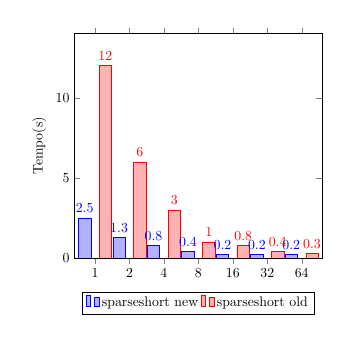
\begin{tikzpicture}[scale=0.5, baseline]
    \begin{axis}[
    %media de tempo new-lee
    width=0.65 \linewidth,
    height=0.6 \linewidth,
    ybar=6pt, 
%    enlargelimits=0.05,
    legend style={at={(0.5,-0.15)}, anchor=north, legend columns=-1},
    ylabel=Tempo(s),
    symbolic x coords={1, 2, 4, 8, 16, 32, 64},
    xtick=data,
    ymin=0,
    ymax=14,
    bar width=9pt,
    nodes near coords,
    nodes near coords align={vertical},
    ]

    \addplot coordinates {(1,2.5) (2,1.3) (4,0.8) (8,0.4) (16,0.2) (32,0.2) (64,0.2)}; %sparseshort
    \addplot coordinates {(1,12) (2,6) (4,3) (8,1) (16,0.8) (32,0.4) (64,0.3)}; %sparseshort old
    \legend {sparseshort new, sparseshort old}
    \end{axis}
\end{tikzpicture}
    }
    
    \subfloat[testboard]{
    \label{ttestboard}
    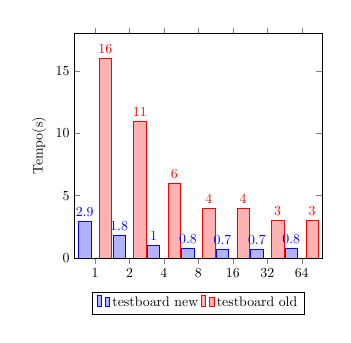
\begin{tikzpicture}[scale=0.5, baseline]
    \begin{axis}[
    %media de tempo old-lee
    width=0.65 \linewidth,
    height=0.6 \linewidth,
    ybar=6pt,
%    enlargelimits=0.12,
    legend style={at={(0.5,-0.15)}, anchor=north, legend columns=-1},
    ylabel=Tempo(s),
    symbolic x coords={1, 2, 4, 8, 16, 32, 64},
    xtick=data,
    ymin=0,
    ymax=18,
    bar width=9pt,
    nodes near coords,
    nodes near coords align={vertical},
    ]

    \addplot coordinates {(1,2.9) (2,1.8) (4,1) (8,0.8) (16,0.7) (32,0.7) (64,0.8)}; %testboard
    \addplot coordinates {(1,16) (2,11) (4,6) (8,4) (16,4) (32,3) (64,3)}; %testboard old
    \legend {testboard new, testboard old}
    \end{axis}
\end{tikzpicture}
    }
    
    \caption{Tempo de execução (s) em NUMA variando o número de \emph{threads}.}
    \label{temp}

\end{figure}